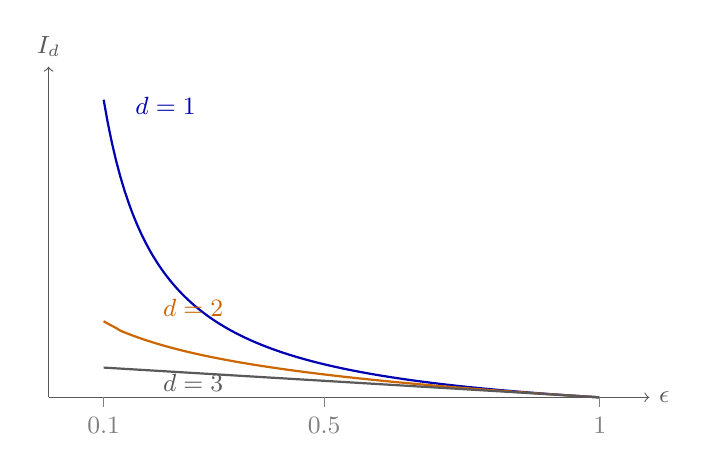
\begin{tikzpicture}[x=7cm,y=0.42cm]
\draw[->,black!65] (0,0)--(1.09,0) node[right,font=\small] {$\epsilon$};
\draw[->,black!65] (0,0)--(0,10) node[above,font=\small] {$I_d$};
\draw[blue!70!black,thick] plot[domain=0.1:1,samples=120] (\x,{1/\x-1});
\draw[orange!80!black,thick] plot[domain=0.1:1,samples=120] (\x,{-ln(\x)});
\draw[black!65,thick] plot[domain=0.1:1,samples=80] (\x,{1-\x});
\node[blue!70!black,font=\small,anchor=west] at (0.14,8.8) {$d=1$};
\node[orange!80!black,font=\small,anchor=west] at (0.19,2.7) {$d=2$};
\node[black!65,font=\small,anchor=west] at (0.19,0.45) {$d=3$};
\foreach \x in {0.1,0.5,1}{\draw[black!50] (\x,0)--(\x,-0.3) node[below,font=\small] {$\x$};}
\end{tikzpicture}
